\documentclass[11pt,a4paper]{article}
\usepackage[margin=2.2cm]{geometry}
\usepackage{amsmath,amssymb}
\usepackage{booktabs}
\usepackage{listings}
\usepackage{xcolor}
\usepackage{hyperref}
\usepackage{tikz}
\usetikzlibrary{positioning,arrows.meta,calc}

\lstset{
  basicstyle=\ttfamily\small,
  keywordstyle=\color{blue!70!black}\bfseries,
  commentstyle=\color{gray},
  stringstyle=\color{orange!70!black},
  numbers=left, numberstyle=\tiny\color{gray},
  frame=single, breaklines=true, columns=fullflexible,
  showstringspaces=false, language=Python,
}

\title{\textbf{AMS/OSRAM AS5048A magnetic rotary encoder}\\[2pt]
       \large Internal notes -- SPI driver, wiring, calibration}
\author{Repo \texttt{exo-actuator-sensor-drivers}}
\date{\today}

\begin{document}\maketitle

% =========================================================================
\section{What it is}
% =========================================================================
The AS5048A is a contactless 360$^{\circ}$ magnetic rotary position
sensor manufactured by AMS / ams~OSRAM Group.  A lateral Hall array on
the chip measures the field of a small diametrically magnetised disc
glued to the rotating shaft above the package; an internal CORDIC
computes the angle and an SPI interface returns it as a 14-bit value.

\begin{center}\small
\begin{tabular}{ll}
\toprule
Property & Value\\
\midrule
Resolution         & 14 bit ($16384$ counts/rev, $0.0219^\circ$/LSB)\\
Sampling rate      & $11.25\,$kHz typ.\\
Propagation delay  & $100\,\mu$s typ.\\
SPI clock          & up to $10\,$MHz (mode~1, CPOL$=0$, CPHA$=1$)\\
Frame length       & 16 bit, MSB first, even parity\\
Supply             & $3.0$--$3.6\,$V (VDD3V) or $4.5$--$5.5\,$V (VDD5V via LDO)\\
Operating temp.    & $-40$ to $+150^{\circ}$C ($5\,$V) / $+125^{\circ}$C ($3.3\,$V)\\
Package            & TSSOP-14 ($5 \times 6.4\,$mm)\\
Magnet             & diametrically magnetised, $\diameter 6$--$8\,$mm, $30$--$70\,$mT at die\\
\bottomrule
\end{tabular}
\end{center}

\paragraph{Variants.}
\textbf{AS5048A} = SPI + PWM, \textbf{AS5048B} = I$^2$C + PWM
(same die, different output pins).  This repo uses the A part on an
AMS evaluation/adapter board, connected via SPI to a Jetson.

% =========================================================================
\section{Wiring: encoder $\to$ Jetson Orin Nano}
% =========================================================================
The encoder adapter board exposes six pins; map them directly to the
SPI0 pins on the Orin Nano 40-pin header:

\begin{center}\small
\begin{tabular}{lll}
\toprule
Encoder pin & Jetson pin & Jetson signal\\
\midrule
\texttt{GND}  & 25 & GND\\
\texttt{3V3}  & 17 & 3.3\,V\\
\texttt{MOSI} & 19 & SPI0\_MOSI\\
\texttt{MISO} & 21 & SPI0\_MISO\\
\texttt{SCK}  & 23 & SPI0\_SCK\\
\texttt{CSN}  & 24 & SPI0\_CS0\\
\bottomrule
\end{tabular}
\end{center}

\noindent This corresponds to the device node \texttt{/dev/spidev0.0}
(verified by the loopback test; see Section~\ref{sec:loopback}).
The SPI pins are tristated by default on every boot and must be
activated via a device tree overlay -- see Section~\ref{sec:overlay}.

\paragraph{Powering.} The adapter board's on-board LDO accepts both
3.3\,V and 5\,V, but the Jetson header is 3.3\,V logic only -- always
power from pin~17.  Do \emph{not} connect 5\,V to a board whose pull-ups
are referenced to 3.3\,V.

% =========================================================================
\section{Enabling SPI on the Jetson: device tree overlay}
\label{sec:overlay}
% =========================================================================
The SPI pads on the 40-pin header are \textbf{tristated (high-Z) by
default} after every boot.  They must be mux'd to the SPI controller
with a pinmux overlay before the kernel driver will accept transfers.

\subsection{Option A -- \texttt{jetson-io.py} (interactive, not used here)}
Run \texttt{sudo /opt/nvidia/jetson-io/jetson-io.py}, select
``Configure Jetson 40pin Header'', toggle ``SPI1'', save and reboot.
This writes a pre-baked DTBO supplied by NVIDIA.  It works for a quick
test but the overlay is untracked and cannot be customised.

\subsection{Option B -- custom DTBO (used in this repo)}
A hand-authored overlay lives at:
\begin{center}
  \texttt{jetson-orin-spi-overlay-guide/examples/as5048a-encoder/}
\end{center}

\textbf{Files in that folder:}
\begin{itemize}
  \item \texttt{jetson-orin-as5048a.dts} -- DTS source.  Configures the
        four Tegra pads\linebreak
        \texttt{spi1\_mosi\_pz5} / \texttt{spi1\_miso\_pz4} /
        \texttt{spi1\_sck\_pz3} / \texttt{spi1\_cs0\_pz6}
        (header pins 19/21/23/24) to function \texttt{spi1}.  No extra
        GPIO fragment is needed because the encoder's CSN is driven by
        hardware CS0.
  \item \texttt{install.sh} -- compiles the DTS with \texttt{dtc},
        copies the DTBO to \texttt{/boot/}, backs up
        \texttt{/boot/extlinux/extlinux.conf} with a timestamp,
        appends a new \texttt{LABEL AS5048A} entry, and sets
        \texttt{DEFAULT AS5048A}.
\end{itemize}

\textbf{Installation:}
\begin{lstlisting}[language=bash]
cd jetson-orin-spi-overlay-guide/examples/as5048a-encoder
chmod +x install.sh
sudo ./install.sh   # compiles DTS, installs DTBO, updates extlinux.conf
# reboot when prompted
\end{lstlisting}

\textbf{What extlinux.conf looks like after the installer runs:}
\begin{lstlisting}[language=bash]
DEFAULT AS5048A

LABEL primary
    LINUX /boot/Image
    APPEND ...

LABEL AS5048A
    LINUX /boot/Image
    FDT   /boot/dtb/kernel_tegra234-p3768-0000+p3767-0005-nv-super.dtb
    INITRD /boot/initrd
    APPEND ...
    OVERLAYS /boot/jetson-orin-as5048a.dtbo
\end{lstlisting}

U-Boot reads this file at boot, loads the base DTB, patches it with
the overlay before handing it to the kernel, and the four SPI pads come
up mux'd.  Confirm pinmux was applied after rebooting:
\begin{lstlisting}[language=bash]
sudo cat /sys/kernel/debug/pinctrl/2430000.pinmux/pinmux-pins \
     | grep -iE "spi1_mosi|spi1_miso|spi1_sck|spi1_cs0"
# expected output (all four lines):
# pin 133 (SPI1_SCK_PZ3):  ... function spi1 group spi1_sck_pz3
# pin 134 (SPI1_MISO_PZ4): ... function spi1 group spi1_miso_pz4
# pin 135 (SPI1_MOSI_PZ5): ... function spi1 group spi1_mosi_pz5
# pin 136 (SPI1_CS0_PZ6):  ... function spi1 group spi1_cs0_pz6
\end{lstlisting}

\paragraph{Reverting.}
Edit \texttt{/boot/extlinux/extlinux.conf} and change
\texttt{DEFAULT AS5048A} to \texttt{DEFAULT primary}, then reboot.
The timestamped backup created by the installer can also be restored
verbatim.

\subsection{Installing the Python \texttt{spidev} binding}
\label{sec:spidev}
The \texttt{spidev} package must be installed \textbf{system-wide} so
that \texttt{sudo python3} (needed because \texttt{/dev/spidev*} is
owned by root/\texttt{gpio}) can find it.
\begin{lstlisting}[language=bash]
sudo pip3 install spidev          # system-wide; do NOT use --user
sudo usermod -aG dialout,gpio,spi $USER  # optional: grant non-root access
# log out and back in for group membership to take effect
\end{lstlisting}

\textbf{Why not \texttt{--user}?}  Running \texttt{pip3 install --user
spidev} installs the package under \texttt{\$HOME/.local}, which is
the calling user's home directory.  When you then run \texttt{sudo
python3}, Python uses \emph{root}'s site-packages -- a different path --
and the import fails with \texttt{FAIL: spidev not installed}.

% =========================================================================
\section{SPI bus mapping and the loopback test}
\label{sec:busmap}
% =========================================================================

\subsection{The Tegra-name vs.~Linux-number confusion}
The Tegra silicon labels the four pads on the 40-pin header
\texttt{spi1\_mosi\_pz5} etc., and the DTS function string is
\texttt{"spi1"} -- which suggests this is Linux SPI bus~1
(\texttt{/dev/spidev1.0}).  It is not.

On the \textbf{Jetson Orin Nano Devkit (P3768)} the kernel probes the
controllers in memory-map order:
\begin{center}\small
\begin{tabular}{lll}
\toprule
Tegra block & Linux name & Device node \\
\midrule
\texttt{spi@3210000} & \texttt{spi0} & \texttt{/dev/spidev\textbf{0}.0} \\
\texttt{spi@3230000} & \texttt{spi1} & \texttt{/dev/spidev\textbf{1}.0} \\
\bottomrule
\end{tabular}
\end{center}

The 40-pin header pins 19/21/23/24 are wired to \texttt{spi@3210000},
so the correct device node is \texttt{/dev/spidev\textbf{0}.0} and the
driver default is \texttt{AS5048AConfig(bus=0, device=0)}.  The pad
names with ``spi1'' in them reflect the \emph{silicon block label}, not
the Linux bus index.

On other Jetson carriers (e.g.\ AGX Orin) the same pads may be wired to
\texttt{spi@3230000} = \texttt{/dev/spidev1.0}.  Always run the
loopback test (\S\ref{sec:loopback}) on an unfamiliar board before
hardcoding \texttt{bus=}.

\subsection{Loopback test methodology}
\label{sec:loopback}

\textbf{What it is.}
An SPI loopback test sends a known byte pattern out of MOSI and reads
back whatever arrives on MISO.  With a physical jumper wire connecting
MOSI to MISO -- and no chip on the bus to drive MISO independently --
the received bytes must exactly match the transmitted bytes, proving
that the SPI controller, the kernel driver, and the physical pin are
all working end-to-end.

\textbf{How to run it.}
\begin{enumerate}
  \item Disconnect the encoder from the header.
  \item Short pin~19 (MOSI) to pin~21 (MISO) with a short jumper wire.
  \item Run: \texttt{sudo python3 tests/encoder/00\_spi\_connectivity.py}
\end{enumerate}
Stage~1 of the script probes both \texttt{/dev/spidev0.0} and
\texttt{/dev/spidev1.0} without any manual input, transmitting the
8-byte test pattern \texttt{A5 5A 12 34 DE AD BE EF}.

\textbf{Expected output with the overlay active and the jumper on
pins~19/21:}
\begin{lstlisting}[language=bash]
Stage 1: SPI loopback test
  /dev/spidev0.0  -- PASS  tx=A5 5A 12 34 DE AD BE EF
                            rx=A5 5A 12 34 DE AD BE EF
  /dev/spidev1.0  -- FAIL  rx all 0x00 (MISO floating)
  -> SPI controller OK.  Remove the jumper and reconnect the encoder.
\end{lstlisting}
\texttt{spidev0.0} echoes perfectly because the MOSI pad is
physically shorted back to the MISO pad.  \texttt{spidev1.0} reads
all~0x00 because that controller is not wired to the 40-pin header on
this board.

\textbf{Failure modes and causes:}
\begin{center}\small
\begin{tabular}{lll}
\toprule
Bus & Result & Cause \\
\midrule
\texttt{spidev0.0} & all 0x00 & overlay not applied; SPI pads still tristated \\
\texttt{spidev0.0} & all 0xFF & MISO pulled high; jumper not making contact \\
\texttt{spidev0.0} & mismatch & wiring error or noisy jumper wire \\
both buses & all 0x00 & not rebooted after \texttt{install.sh}, or \texttt{extlinux.conf}\\
           &          & \texttt{DEFAULT} not set to \texttt{AS5048A} \\
\bottomrule
\end{tabular}
\end{center}

\textbf{After the loopback passes:} remove the jumper, reconnect the
encoder, and run Stage~2 of the script.  A live chip (even without a
magnet) returns non-zero words at all three test speeds
(100\,kHz / 500\,kHz / 1\,MHz); all-zero means a wiring or power problem.

% =========================================================================
\section{SPI protocol}
% =========================================================================
Every transaction is a 16-bit MSB-first frame.  CSn falls, 16 clocks
shift, CSn rises.  At least $350\,$ns must elapse between two CSn pulses
(\texttt{tCSnH}); between frames the master typically idles the bus.

\subsection{Frame formats}

\textbf{Command} (master $\to$ AS5048A):
\[
\boxed{\,[\text{PAR}_{15}] \;[\text{RWn}_{14}] \;[\text{addr}_{13\ldots 0}]\,}
\]
where \texttt{RWn} = 1 for read, 0 for write.  Parity is \textbf{even}
over bits 0--14: the parity bit is chosen so the total number of 1s in
the 16-bit frame is even.

\textbf{Response} (AS5048A $\to$ master):
\[
\boxed{\,[\text{PAR}_{15}] \;[\text{EF}_{14}] \;[\text{data}_{13\ldots 0}]\,}
\]
\texttt{EF}~$=$~1 means an error occurred in the \emph{previous} host
frame (parity / unknown command / wrong number of clocks).  Read
register \texttt{0x0001} (``Clear Error Flag'') to find out which.

\textbf{Write data} (master $\to$ AS5048A on the cycle following a
write command):
\[
\boxed{\,[\text{PAR}_{15}] \;[R_{14}=0] \;[\text{data}_{13\ldots 0}]\,}
\]

\subsection{Read sequence (latency of one frame)}
\begin{center}
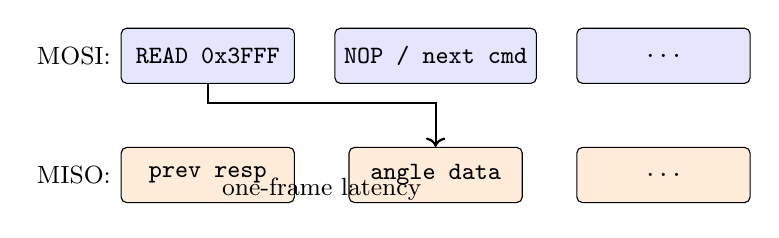
\begin{tikzpicture}[node distance=4mm and 5mm,
                    every node/.style={font=\small\ttfamily},
                    box/.style={draw,rounded corners=2pt,
                                minimum width=2.2cm,minimum height=7mm,fill=blue!10}]
  \node[box] (cmd)  {READ 0x3FFF};
  \node[box,right=of cmd] (nop)  {NOP / next cmd};
  \node[box,right=of nop] (more) {\ldots};

  \node[box,fill=orange!15,below=8mm of cmd]  (r1) {prev resp};
  \node[box,fill=orange!15,below=8mm of nop]  (r2) {angle data};
  \node[box,fill=orange!15,below=8mm of more] (r3) {\ldots};

  \draw[->,thick] (cmd)  -- ++(0,-6mm) -| (r2);
  \node[font=\small] at ($(cmd)!.5!(nop) + (0,-1.7cm)$) {one-frame latency};

  \node[font=\small,left=0pt of cmd]  {MOSI:};
  \node[font=\small,left=0pt of r1]   {MISO:};
\end{tikzpicture}
\end{center}

\noindent Send the READ command, then any next frame (typically NOP);
the response containing the requested register sits in the MISO of that
\emph{second} frame.

\subsection{Register map (relevant subset)}
\begin{center}\small
\begin{tabular}{lll}
\toprule
Address & Name & Notes\\
\midrule
\texttt{0x0000} & NOP                & response = 0; used as filler\\
\texttt{0x0001} & Clear Error Flag   & read $\to$ clears EF, returns error bits\\
\texttt{0x0003} & Programming Control& Verify / Burn / Programming~Enable\\
\texttt{0x0016} & OTP zero pos hi    & bits $\langle 13\!:\!6\rangle$ of zero offset\\
\texttt{0x0017} & OTP zero pos lo    & bits $\langle 5\!:\!0\rangle$ of zero offset\\
\texttt{0x3FFD} & Diag + AGC         & OCF, COF, COMP\_low, COMP\_high, AGC$\langle 7\!:\!0\rangle$\\
\texttt{0x3FFE} & Magnitude          & CORDIC magnitude (proxy for $|B_z|$)\\
\texttt{0x3FFF} & Angle              & zero-corrected 14-bit angle\\
\bottomrule
\end{tabular}
\end{center}

\subsection{Error register bits (response to \texttt{0x0001})}
\begin{center}\small
\begin{tabular}{lll}
\toprule
Bit & Name & Meaning\\
\midrule
2 & Parity Error    & host parity wrong\\
1 & Command Invalid & unknown address / RWn combination\\
0 & Framing Error   & not exactly 16 clocks between CSn edges\\
\bottomrule
\end{tabular}
\end{center}

% =========================================================================
\section{Driver layout in this repo}
% =========================================================================
Mirror of the Damiao layout (see \texttt{docs/notes/dm\_j4310\_notes.tex}):

\begin{itemize}
  \item \texttt{src/encoder\_config.py} -- single source of truth for SPI
        wiring.  Exposes \texttt{AS5048AConfig(bus, device, max\_hz, mode)}
        and \texttt{DEFAULT\_ENCODER\_CONFIG = AS5048AConfig(0, 0,
        1\,000\,000, 1)}.
  \item \texttt{src/as5048a.py} -- the \texttt{AS5048A} class.  Provides
        \texttt{connect}, \texttt{disconnect}, \texttt{is\_connected},
        \texttt{\_\_enter\_\_}/\texttt{\_\_exit\_\_},
        \texttt{read\_angle\_raw}/\texttt{\_deg}/\texttt{\_rad},
        \texttt{read\_magnitude}, \texttt{read\_diagnostics},
        \texttt{set\_zero}, plus the low-level \texttt{read\_register} /
        \texttt{write\_register} primitives.
  \item \texttt{tests/encoder/} -- numbered test scripts (see below).
\end{itemize}

\subsection{Test scripts: summary}
\begin{center}\small
\begin{tabular}{ll}
\toprule
File & Purpose\\
\midrule
\texttt{00\_spi\_connectivity.py} & SPI loopback + raw chip probe; run first on a new board\\
\texttt{01\_read\_angle.py}       & 50\,Hz print loop of raw / deg / rad\\
\texttt{02\_diagnostics.py}       & AGC, magnitude and verdict on magnet placement\\
\texttt{03\_set\_zero.py}         & latch current angle as zero (RAM only by default)\\
\texttt{04\_zero\_and\_track.py}  & zero current position, then track rotation with direction\\
\bottomrule
\end{tabular}
\end{center}

\subsection{Minimal usage}
\begin{lstlisting}
from encoder_config import DEFAULT_ENCODER_CONFIG
from as5048a import AS5048A

with AS5048A(DEFAULT_ENCODER_CONFIG) as enc:
    print(enc.read_angle_deg())            # 0..360 degrees
    print(enc.read_diagnostics())          # {'agc': 128, 'ocf': 1, ...}
    enc.set_zero(burn_otp=False)           # latch current pose as 0
\end{lstlisting}

% =========================================================================
\section{Test scripts walkthrough -- every SPI byte explained}
\label{sec:walkthrough}
% =========================================================================
This section is a line-by-line audit of the four scripts in
\texttt{tests/encoder/}.  For each script we list the exact bytes that
travel on MOSI/MISO, decode every response, and explain what each
field means in the firmware.

\medskip
\noindent\textbf{Notation used below.}
\begin{itemize}
  \item All SPI frames are 16-bit MSB-first.  Python's \texttt{spidev}
        operates on 8-bit lists, so a frame is sent as two bytes
        \texttt{[hi, lo]}.
  \item A \textbf{read} of address \texttt{A} requires two SPI frames:
        the first carries the READ command, the second carries any
        next command and \emph{returns} the data in its MISO bytes.
        This is the ``one-frame latency'' from
        \S\ref{sec:loopback}.
  \item Command word layout:
        \texttt{[PAR\textsubscript{15} | RWn\textsubscript{14} |
        addr\textsubscript{13..0}]}.  \texttt{PAR} is even parity over
        bits 0..14, \texttt{RWn}=1 for read.
  \item Response word layout:
        \texttt{[PAR\textsubscript{15} | EF\textsubscript{14} |
        data\textsubscript{13..0}]}.  \texttt{EF}=1 means an error
        occurred in the \emph{previous} host frame.
\end{itemize}

% -------------------------------------------------------------------------
\subsection{\texttt{00\_spi\_connectivity.py} -- wiring \& chip check}
% -------------------------------------------------------------------------
Run this on a freshly-flashed Jetson with the overlay installed but
before connecting any application code.  It is divided into four stages
and is the only script that bypasses the high-level driver and pokes
\texttt{spidev} directly.

\paragraph{Stage 0: enumerate \texttt{/dev/spidev*}.}
A simple \texttt{glob.glob("/dev/spidev*")}.  Expected on a Devkit:
\texttt{[/dev/spidev0.0, /dev/spidev0.1, /dev/spidev1.0,
/dev/spidev1.1]}.  Missing nodes mean the overlay did not load (or
\texttt{DEFAULT AS5048A} is not set in \texttt{extlinux.conf}).

\paragraph{Stage 1: SPI loopback.}
\begin{lstlisting}
test_pattern = [0xA5, 0x5A, 0x12, 0x34, 0xDE, 0xAD, 0xBE, 0xEF]
rx = spi.xfer2(list(test_pattern))
\end{lstlisting}
With pins~19 and~21 shorted, the SPI shift register clocks each MOSI
byte out and immediately samples it back on MISO -- so
\texttt{rx == test\_pattern} byte-for-byte.

\textbf{Three possible outcomes per bus:}
\begin{center}\small
\begin{tabular}{lll}
\toprule
\texttt{rx} pattern & Meaning & Action \\
\midrule
\texttt{A5 5A 12 34 DE AD BE EF} & PASS  -- controller works  & remove jumper \\
\texttt{00 00 00 00 \ldots}      & MISO floating              & jumper not seated, or overlay missing \\
\texttt{FF FF FF FF \ldots}      & MISO pulled high           & wrong bus, no chip, no jumper \\
\texttt{any other bytes}         & encoder is driving MISO    & expected when chip is connected \\
\bottomrule
\end{tabular}
\end{center}
The ``MISMATCH'' branch in the script prints a hint that this is
\emph{expected} when the encoder is connected: the chip drives MISO
with its own response (typically the previous-frame data for whatever
\texttt{0xA55A}/\texttt{0x1234}/\ldots\ commands happen to decode as).

\paragraph{Stage 2: live-chip probe at three speeds.}
For each bus and each clock (100/500/1000\,kHz) the script sends a
single READ-DIAG command and collects the response:
\begin{lstlisting}
spi.xfer2([0x7F, 0xFD])           # READ 0x3FFD
rx = spi.xfer2([0xFF, 0xFF])      # collect; payload is 0xFFFF (NOP'ish)
word = (rx[0] << 8) | rx[1]
\end{lstlisting}
\textbf{Why \texttt{0x7FFD}?}
Address \texttt{0x3FFD} | \texttt{RWn=1} (bit~14) = \texttt{0x7FFD}.  We
compute its even parity:
\begin{center}\small
\(0x7FFD = 0111\,1111\,1111\,1101_2\) has 14 one-bits in positions
0..14 $\Rightarrow$ parity = 0 $\Rightarrow$ PAR bit stays 0
$\Rightarrow$ frame = \texttt{0x7FFD}.
\end{center}
\textbf{Interpreting the response.}  Three classes:
\begin{center}\small
\begin{tabular}{ll}
\toprule
Response & Meaning \\
\midrule
\texttt{0x0000} & MISO held low; no chip / wrong bus \\
\texttt{0xFFFF} & MISO pulled high; no chip \\
anything else   & LIVE -- chip is responding \\
\bottomrule
\end{tabular}
\end{center}

\paragraph{Stage 3: parse the DIAG+AGC register.}
On the live bus the script issues:
\begin{enumerate}
  \item \texttt{[0x40, 0x01]}: READ 0x0001 ``Clear Error Flag'' --
        wipes any sticky \texttt{EF} from previous transactions.
        (\texttt{0x0001 | 0x4000} = \texttt{0x4001}; even parity = 0.)
  \item \texttt{[0xFF, 0xFF]}: dummy NOP that collects the error-flag
        response and discards it.
  \item \texttt{time.sleep(0.1)}: 100\,ms wait -- the chip's
        \emph{Offset Compensation Finished} bit (OCF) only sets ${\sim}10\,$ms
        after VDD stabilises, and an OCF retry loop polls a further
        500\,ms if it is still 0.
  \item Eight diag reads, then a re-poll loop if OCF=0.
\end{enumerate}

\textbf{Decoding the response word.}  Given a 16-bit \texttt{word}:
\[
\underbrace{\text{PAR}_{15}}_{1\text{ bit}}\;
\underbrace{\text{EF}_{14}}_{1\text{ bit}}\;
\underbrace{\text{COMPHI}_{11}}_{}\;
\underbrace{\text{COMPLO}_{10}}_{}\;
\underbrace{\text{COF}_{9}}_{}\;
\underbrace{\text{OCF}_{8}}_{}\;
\underbrace{\text{AGC}_{7..0}}_{8\text{ bits}}
\]
\textbf{Worked example.}  Field-test reading on this bench
(no magnet, properly powered):
\begin{center}\small
\(\texttt{0x88FF} = 1000\,1000\,1111\,1111_2\)
\end{center}
\begin{center}\small
\begin{tabular}{lll}
\toprule
Bits & Decoded & Meaning \\
\midrule
$15$    & PAR    = 1 & valid (frame has even number of 1-bits overall) \\
$14$    & EF     = 0 & no error in the previous host frame \\
$11$    & COMPHI = 1 & magnetic field too weak (no magnet present) \\
$10$    & COMPLO = 0 & field not too strong \\
$9$     & COF    = 0 & CORDIC has not overflowed \\
$8$     & OCF    = 0 & offset compensation did \emph{not} complete \\
$7..0$  & AGC    = $0xFF=255$ & gain saturated (no signal to amplify) \\
\bottomrule
\end{tabular}
\end{center}
\textbf{Interpretation:} the chip is fully alive and the SPI framing
is correct (EF=0, valid parity).  AGC=255 + COMPHI=1 says ``no
magnetic field detected'' -- which is the expected state when the test
is run without a magnet present.  OCF=0 is the only ambiguous bit; in
practice the AS5048A frequently leaves OCF=0 until a usable field
appears, because the offset-compensation routine relies on the Hall
sensors having a real signal to null.  Placing the magnet typically
flips OCF to 1 and drops AGC into the 100--200 range.

\textbf{Stage 3 PASS criterion (after magnet placement):}
\begin{center}\small
OCF = 1, COMPHI = 0, COMPLO = 0, AGC $\approx$ 128.
\end{center}

% -------------------------------------------------------------------------
\subsection{\texttt{01\_read\_angle.py} -- continuous angle readout}
% -------------------------------------------------------------------------
The shortest script -- a 50\,Hz print loop that wraps the high-level
driver:
\begin{lstlisting}
with AS5048A(DEFAULT_ENCODER_CONFIG) as enc:
    while True:
        raw = enc.read_angle_raw()
        deg = raw * (360.0 / 16384.0)
        rad = raw * (6.283185307179586 / 16384.0)
        print(f"\r{raw:5d}  {deg:7.3f}  {rad:7.4f}", end="", flush=True)
        time.sleep(0.02)
\end{lstlisting}

\textbf{What \texttt{read\_angle\_raw()} does internally.}
\begin{enumerate}
  \item Builds the READ-ANGLE command:
        \(\texttt{0x3FFF} | \texttt{0x4000} = \texttt{0x7FFF}\).
        Its 16-bit population count is 15 (odd over bits 0..14, so
        parity bit = 1) $\Rightarrow$ final command = \texttt{0xFFFF}.
  \item Sends frame 1: \texttt{[0xFF, 0xFF]}.  (Coincidentally
        identical to a NOP-style filler.)  The MISO bytes of this
        frame contain whatever the previous read had latched and are
        discarded.
  \item Sends frame 2: another READ-NOP \texttt{0x4000} command,
        which carries even parity = 0 $\Rightarrow$ bytes
        \texttt{[0x40, 0x00]}.  The MISO of frame~2 now contains the
        angle.
  \item Returns \texttt{word \& 0x3FFF} -- strips PAR and EF, keeps
        the 14-bit value.
\end{enumerate}

\textbf{Scaling.}  $16384$ counts/rev (=\,$2^{14}$):
\(\text{deg} = \text{raw}\cdot 360/16384,\;
\text{rad} = \text{raw}\cdot 2\pi/16384.\)

\textbf{Expected behaviour.}  With a magnet in place and OCF=1, the
\texttt{raw} value smoothly walks through 0..16383 as the shaft turns.
The 14-bit value wraps at $16383 \to 0$ in one LSB ($0.022^{\circ}$).
Without a magnet the angle register still returns a number, but it is
dominated by Hall noise and jumps around -- this is normal.

\paragraph{Parity-check note.}  \texttt{read\_register()} in the
driver currently calls \texttt{\_even\_parity(resp)} which XOR-folds
only bits 0..14 of the response.  Per the datasheet, the response is
\emph{valid} when the full 16-bit count is even (i.e.\ PAR + popcount
of bits 0..14 $\equiv 0$).  A frame like \texttt{0x88FF} (PAR=1,
payload with 9 ones $\Rightarrow$ odd) is valid, but the current code
treats odd payload as an error.  If \texttt{01\_read\_angle.py} raises
sporadic ``AS5048A parity error'' exceptions, fix
\texttt{\_even\_parity} to XOR-fold all 16 bits and require the result
to be 0.

% -------------------------------------------------------------------------
\subsection{\texttt{02\_diagnostics.py} -- AGC + magnet placement check}
% -------------------------------------------------------------------------
A 5\,Hz print loop that prints the DIAG register plus the
\texttt{MAGNITUDE} register (0x3FFE), then verbal verdict:
\begin{lstlisting}
diag = enc.read_diagnostics()
mag  = enc.read_magnitude()
if diag["comp_low"]:   verdict = "FIELD TOO STRONG - increase air gap"
elif diag["comp_high"]: verdict = "FIELD TOO WEAK   - decrease air gap"
elif diag["cof"]:      verdict = "CORDIC OVERFLOW  - check magnet alignment"
elif not diag["ocf"]:  verdict = "offset comp not finished (wait...)"
else:                  verdict = "OK"
\end{lstlisting}

\textbf{SPI traffic per loop iteration.}  Two reads, four frames:
\begin{center}\small
\begin{tabular}{llll}
\toprule
\# & Direction & Bytes (hex) & Meaning \\
\midrule
1 & MOSI & \texttt{7F FD} & READ 0x3FFD \\
1 & MISO & --              & previous-frame data (discarded) \\
2 & MOSI & \texttt{C0 00} & NOP (\texttt{0x0000} as a READ \(=\texttt{0x4000}\); PAR=1) \\
2 & MISO & \texttt{XX XX} & DIAG word -- see decode table above \\
3 & MOSI & \texttt{7F FE} & READ 0x3FFE \\
3 & MISO & --              & previous DIAG data (discarded) \\
4 & MOSI & \texttt{C0 00} & NOP \\
4 & MISO & \texttt{YY YY} & 14-bit magnitude (CORDIC) \\
\bottomrule
\end{tabular}
\end{center}

\textbf{Magnitude register.}  A 14-bit unsigned value proportional to
$\sqrt{B_x^2 + B_y^2}$.  In a well-placed setup it sits in roughly
$2000\!-\!4000$; when the magnet is far away it drops near zero, when
the chip is saturated it pegs near $0x3FFF$.  It is informational only
-- the firmware does not use it to gate the angle output.

\textbf{Tuning workflow:}
\begin{enumerate}
  \item Start with magnet 2--3\,mm above the chip centred on the die.
  \item Lower until \texttt{COMP\_HI} flips from 1 to 0.
  \item Continue lowering; if \texttt{COMP\_LO} sets, you have over-
        shot -- raise back up.
  \item Aim for AGC $\approx 128$.  An AGC of 64--192 is excellent;
        outside 32--224 means re-seat the magnet.
\end{enumerate}

% -------------------------------------------------------------------------
\subsection{\texttt{03\_set\_zero.py} -- programming the OTP zero}
% -------------------------------------------------------------------------
Programs registers 0x0016 / 0x0017 in RAM so the angle register
returns 0 at the current mechanical pose.  By default the change is
volatile (lost on power cycle); pass \texttt{burn\_otp=True} to fuse
it permanently into OTP -- this is irreversible and can be done only
once per chip.

\textbf{Algorithm (datasheet ``Programming Sequence with
Verification'').}
\begin{enumerate}
  \item Write 0 to ZERO\_HI (\texttt{0x0016}) and ZERO\_LO
        (\texttt{0x0017}).  This zeroes any pre-existing offset so the
        next read returns the absolute mechanical angle.
  \item Read the angle register \texttt{0x3FFF}.
  \item Write angle$\langle 13\!:\!6\rangle$ to ZERO\_HI and
        angle$\langle 5\!:\!0\rangle$ to ZERO\_LO.  The chip
        subtracts this 14-bit value from every subsequent angle
        reading.
\end{enumerate}

\textbf{Write-frame layout reminder.}  A write costs three SPI frames:
\begin{center}\small
\begin{tabular}{lll}
\toprule
Frame & MOSI bytes (e.g.\ write \texttt{0x05} to 0x0016) & Meaning \\
\midrule
1 & \texttt{00 16}  & write-command (RWn=0, addr 0x0016, parity 0)\\
2 & \texttt{80 05}  & data word \texttt{0x0005} + parity = \texttt{0x8005} \\
3 & \texttt{C0 00}  & NOP (\texttt{0x4000} | PAR) -- flushes verify response \\
\bottomrule
\end{tabular}
\end{center}
The verify byte returned in frame~3's MISO is the value just written,
echoed by the chip.

\textbf{Example session.}
\begin{lstlisting}[language=bash]
Angle before zeroing : 187.404 deg
Latched offset       :  8528 counts (187.404 deg)
Angle after zeroing  :   0.022 deg     # one-LSB residual is normal
\end{lstlisting}

\textbf{OTP burn (only if \texttt{burn\_otp=True}).}  After step~3:
\begin{enumerate}
  \item Write \texttt{0x01} to PROG\_CONTROL (0x0003) -- Programming
        Enable.
  \item Write \texttt{0x08} to PROG\_CONTROL -- Burn.  Wait 20\,ms.
  \item Read the angle (should now be 0).
  \item Write \texttt{0x40} to PROG\_CONTROL -- Verify (re-loads OTP).
\end{enumerate}
\textbf{Important:} the OTP fuses can be programmed exactly once.  Burn
only when the mechanical mounting is finalised.

% -------------------------------------------------------------------------
\subsection{\texttt{04\_zero\_and\_track.py} -- zero then track rotation}
% -------------------------------------------------------------------------
This script combines the zeroing step with a live 50\,Hz tracking loop.
It is the primary script for verifying encoder behaviour on a mounted
joint.

\textbf{What it does:}
\begin{enumerate}
  \item Reads the current raw angle and prints it.
  \item Calls \texttt{enc.set\_zero(burn\_otp=False)} to latch that
        angle as the new zero in RAM (volatile -- lost on power cycle).
  \item Enters a 50\,Hz loop printing:
        \begin{itemize}
          \item \texttt{raw} -- 14-bit count (0..16383).
          \item \texttt{deg} -- angle relative to zero, wrapped to
                $(-180^{\circ}, +180^{\circ}]$.
          \item \texttt{rad} -- same in radians.
          \item \texttt{dir} -- \texttt{CCW} or \texttt{CW} vs.\ previous
                sample.
          \item \texttt{total\_deg} -- cumulative signed rotation (can
                exceed $\pm 360^{\circ}$ for multi-turn tracking).
        \end{itemize}
  \item On Ctrl+C: prints total rotation summary.
\end{enumerate}

\textbf{Signed-delta algorithm.}  Because the 14-bit counter wraps at
$16383 \to 0$, a naive difference would give a spurious $-16383$ count
when crossing the wrap boundary.  The script uses the shortest-arc
algorithm:
\begin{lstlisting}
def signed_delta(a, b):
    d = (b - a) % 16384          # always positive
    if d > 8192: d -= 16384      # fold into (-8192, +8192]
    return d                     # positive = CCW, negative = CW
\end{lstlisting}
This is correct for any single-sample step smaller than a half-turn
(8192 counts = $180^{\circ}$), which is guaranteed at 50\,Hz unless
the shaft spins faster than $50 \times 180^{\circ}/\text{s}$ =
$25\,\text{rev/s}$ = $1500\,\text{rpm}$.

\textbf{Error-flag auto-retry.}  During a live run at 50\,Hz over
jumper wires, the chip's \texttt{EF} (error flag) bit occasionally
sets due to SPI bus noise triggering a spurious host-parity error in
the chip.  \texttt{read\_register()} in \texttt{as5048a.py} clears EF
and retries the read once before raising, so the loop runs
uninterrupted.  If EF persists on both attempts a real error is raised.

\textbf{Example session (bench run, magnet on motor shaft):}
\begin{lstlisting}[language=bash]
Connected to /dev/spidev0.0 @ 1.0 MHz, mode 1

Current angle :  3624 counts  ( 79.629 deg)
Zero latched  :  7395 counts  (162.488 deg offset)
Angle now     :   327 counts  (  7.185 deg)  (should be ~0)

Rotate the magnet.  Ctrl+C to stop.

   raw        deg       rad   dir   total_deg
--------------------------------------------------
 14683    -37.375   -0.6523    CW    -764.978
\end{lstlisting}
In this run the magnet was rotated roughly $-765^{\circ}$ (about
$-2.1$ turns CW) before the script was stopped.

\textbf{Startup note.}  The first time \texttt{set\_zero} writes 0 to
0x0016/0x0017 and reads back the angle, the result may be a few counts
off zero due to the one-frame SPI latency -- a residual of
$\leq 3^{\circ}$ is normal and does not affect tracking accuracy.

% =========================================================================
\section{Calibration: zero-position and magnet placement}
% =========================================================================
\subsection{Why zero matters}
The chip's encoder is absolute, but the mechanical zero of your joint
will rarely coincide with the chip's internal zero.  Setting the
\textbf{OTP zero registers} (0x0016/0x0017) makes the angle register
return 0 at the desired mechanical pose, with no software offset
maintained host-side.

\subsection{Programming sequence (RAM, reversible)}
This is what \texttt{enc.set\_zero(burn\_otp=False)} executes:
\begin{enumerate}
  \item Write 0 to 0x0016 \emph{and} 0x0017 -- this clears any existing
        offset, so the next read returns the absolute mechanical angle.
  \item Read the angle register 0x3FFF.
  \item Split the 14-bit value: bits $\langle 13\!:\!6\rangle$ to
        0x0016, bits $\langle 5\!:\!0\rangle$ to 0x0017.
\end{enumerate}
The offset survives until power-cycle.

\subsection{Permanent OTP burn (one-shot, irreversible)}
After the steps above, set the Programming Enable bit (0x01) and then
the Burn bit (0x08) in 0x0003, verify (0x40), and re-read.  The OTP
fuses can be burned \textbf{only once}.  Use \texttt{burn\_otp=True} in
the driver \emph{only} when you are sure of the mechanical mounting.

\subsection{Magnet placement}
The datasheet specifies a magnetic flux of $30$--$70\,$mT perpendicular
to the die surface, at the chip centre.  Practical checks:
\begin{itemize}
  \item Use a $\diameter 6$--$8\,$mm, $\geq 2.5\,$mm thick diametrically
        magnetised disc magnet (NdFeB or SmCo).
  \item Maintain $0.5$--$2.5\,$mm air gap from package surface.
  \item Centre the magnet over the package within
        $R_d \leq 0.25\,$mm displacement (larger magnets allow up to
        $0.5\,$mm).
  \item Monitor the diagnostic flags:
        \texttt{comp\_low}=1 $\Rightarrow$ field too strong,
        \texttt{comp\_high}=1 $\Rightarrow$ field too weak.
        Target AGC near 128.
\end{itemize}

% =========================================================================
\section{Common gotchas}
% =========================================================================
\begin{enumerate}
  \item \textbf{SPI mode is 1}, not 0.  The datasheet wording ``MOSI on
        falling CLK, MISO on rising CLK'' = CPOL=0, CPHA=1.  With mode~0
        you read garbage.
  \item \textbf{Two frames per read.}  The response to a READ command
        lands in the \emph{next} frame; the very first response after
        power-up is undefined.  Discard it or send a dummy first read.
  \item \textbf{Error flag is sticky.}  Once EF is set, every subsequent
        response carries it until you issue Clear Error Flag (0x0001).
        The driver does this automatically on \texttt{connect()}.
  \item \textbf{Parity is even, not odd.}  XOR-fold bits 0..14, place
        the result in bit~15.
  \item \textbf{Jumper-wire layouts.}  Keep MISO/SCK short on a
        breadboard; >5\,MHz over loose wires will give framing errors
        that surface as the EF bit.  The driver default of 1\,MHz is
        deliberately conservative.
  \item \textbf{Permission to access \texttt{/dev/spidev0.0}.}  The
        device node is owned by root and group \texttt{gpio} (mode
        \texttt{660}).  Use \texttt{sudo python3} or add yourself to
        the \texttt{gpio}/\texttt{spi} groups and log out/in.
  \item \textbf{\texttt{spidev} must be installed system-wide for
        \texttt{sudo}.}  \texttt{pip3 install --user spidev} installs
        under \texttt{\$HOME/.local} which is invisible to root's
        Python.  Always use \texttt{sudo pip3 install spidev} (no
        \texttt{--user}) so that \texttt{sudo python3} can import it.
        See Section~\ref{sec:spidev}.
  \item \textbf{Linux bus number $\ne$ Tegra pad label.}  The pads are
        named \texttt{spi1\_*\_pz*} in silicon and the DTS, but on the
        Orin Nano Devkit the 40-pin header routes to
        \texttt{spi@3210000} = \texttt{/dev/spidev\textbf{0}.0}.
        Always verify with the loopback test
        (\texttt{00\_spi\_connectivity.py}) on any new board.
\end{enumerate}

% =========================================================================
\section{Useful references}
% =========================================================================
\begin{itemize}
  \item \texttt{docs/Encoder-AS5048.pdf} -- the datasheet
        (v1-11, 2018-Jan-29).
  \item \texttt{src/as5048a.py} -- this repo's driver, used by
        \texttt{tests/encoder/}.
  \item \emph{spidev} (\url{https://github.com/doceme/py-spidev}) --
        the Python SPI binding used here.
  \item \emph{iotexpert/AS5048A\_Python} -- minimal Python implementation
        for Linux SBCs (good reference for parity logic).
  \item \emph{RobTillaart/AS5048A} -- Arduino C++ port, well-commented;
        useful sanity check on register access timing.
  \item ODrive firmware (\url{https://github.com/odriverobotics/ODrive})
        contains a production-quality C driver for the closely related
        AS5047, which speaks the same 16-bit even-parity SPI frame.
\end{itemize}

\end{document}
